\documentclass[11pt,a4paper]{article}
\usepackage[margin=1in]{geometry}
\usepackage{enumitem}
\usepackage{booktabs}
\usepackage{hyperref}
\usepackage{graphicx}
\usepackage{titling}
\usepackage{xcolor}
\usepackage{amssymb}
\usepackage{tikz}
\usetikzlibrary{shapes.geometric,arrows.meta,positioning,calc}
\newcommand{\todo}[1]{\textbf{\textcolor{red}{[TODO: #1]}}}
\newcommand{\blank}{\vspace{2em}}

\setlength{\droptitle}{-2em}
\pretitle{\begin{center}\Large\bfseries}
\posttitle{\end{center}\vspace{-1em}}

\title{GrandOMR: Interactive Orchestral Score Recognition and Playback}
\author{
  \textsc{Zihan Guo} \\ \texttt{2024011317} \and
  \textsc{Chengwei Liang} \\ \texttt{2024010681}
}
\date{Computer Vision, Spring 2026}

\begin{document}
\maketitle

% ─────────────────────────────────────────────────────────────────────────────
\section{Introduction}
% ─────────────────────────────────────────────────────────────────────────────

% - Background: massive IMSLP scanned scores; limitations of existing OMR systems
%   (Audiveris breaks at low resolution; homr/LEGATO lose instrument identity)
% - Core challenge: orchestral score OMR is heterogeneous across subproblems —
%   structural detection / semantic recognition / symbol classification /
%   temporal alignment each have different characteristics
% - Contribution: match each subproblem to the most suitable CV method,
%   assembling a hybrid pipeline that is interpretable and controllable
% - Paper structure

The International Music Score Library Project (IMSLP)~\cite{imslp} hosts tens of thousands of high-resolution scans of orchestral scores spanning several centuries of repertoire.
Converting these images into machine-readable symbolic music — a task known as Optical Music Recognition (OMR) — would enable large-scale musicological analysis, interactive playback, and digital preservation.
Yet existing OMR systems fall short in the orchestral setting: rule-based engines such as Audiveris~\cite{audiveris} degrade sharply at moderate scan resolution and struggle with printing artifacts; neural staff-level systems such as homr~\cite{oemer} recognise notes accurately but discard all instrument identity; and end-to-end vision-language models such as LEGATO~\cite{legato} are constrained by output-length limits that preclude full orchestral pages.

The fundamental difficulty is that orchestral score OMR is not a single, homogeneous problem.
Staff and system boundary detection is a geometric layout task; instrument name reading must handle multilingual abbreviations and label-to-staff ambiguity; note recognition is a sequence transduction problem with rich rhythmic and pitch relationships; cross-part consistency requires reasoning about musical constraints that are well-defined but vary globally; and dynamics detection amounts to localising a small fixed set of glyph classes amid expressive text.
Each subproblem has a different input distribution, output space, and failure mode.
A monolithic end-to-end model must simultaneously master all of these, which forces compromises on every front.

We present \textbf{GrandOMR}, a hybrid pipeline that decomposes orchestral score OMR into its constituent subproblems and matches each to the most appropriate computer vision method: semantic segmentation (SegNet) for staff and symbol detection, a two-pass vision-language model (VLM) for instrument name identification, a Transformer sequence model (TrOMR) for per-staff note recognition, rule-based post-processing for cross-part structural repair, and a fine-tuned object detector (YOLOv8n) for dynamics detection.
This design keeps each component interpretable and controllable, makes it straightforward to replace individual stages as better models become available, and collectively achieves competitive accuracy on full orchestral scores.

The remainder of the paper is organised as follows.
Section~2 reviews related work.
Section~3 gives a system overview.
Section~4 describes each pipeline stage in detail.
Section~5 reports experimental results.
Sections~6 and~7 discuss limitations and conclude.


% ─────────────────────────────────────────────────────────────────────────────
\section{Related Work}
% ─────────────────────────────────────────────────────────────────────────────

\subsection{Rule-based OMR: Audiveris}
% 20-step rule-based pipeline; template matching + shallow neural classifier;
% high-resolution requirement; lacks robustness to printing artifacts

Audiveris~\cite{audiveris} is an open-source OMR engine built around a roughly twenty-step rule-based pipeline that combines staff-line detection, symbol template matching, and a shallow neural classifier for glyph recognition.
Its architecture is highly interpretable and produces well-formed MusicXML output for clean engraved scores.
However, it imposes stringent image quality requirements: recognition accuracy degrades markedly below approximately 300~DPI, and it is sensitive to printing artifacts, page curvature, and ink bleed-through that are common in IMSLP scans.
Audiveris also provides reasonable instrument name extraction from score headers, but it was designed primarily for single-instrument or small-ensemble scores and lacks robust handling of the complex bracket and brace structures found in full orchestral layouts.

\subsection{Neural Staff-level OMR: TrOMR / homr}
% TrOMR: Transformer encoder-decoder at staff level (ICASSP 2023)
% homr: UNet segmentation front-end + TrOMR; no instrument identity

TrOMR~\cite{tromr} is a Transformer-based encoder-decoder that treats per-staff music recognition as a sequence transduction problem: given a cropped staff image, it outputs a linearised token sequence encoding pitch, duration, accidentals, and articulations.
By operating at the staff level, TrOMR sidesteps the complexity of multi-staff layout and achieves strong symbol-error rates on standard benchmarks.
The homr system~\cite{oemer} augments TrOMR with a UNet-based semantic segmentation front-end that detects staves, noteheads, stems, clefs, and barlines, enabling fully automatic end-to-end recognition from raw page images.
However, neither system recovers instrument identity: homr assigns generic part labels and provides no mechanism for cross-page name propagation, making it unsuitable for producing playback-ready orchestral scores.

\subsection{Large-scale End-to-end OMR: LEGATO}
% Frozen LLaMA 3.2 vision encoder + ABC-notation decoder; SOTA on piano/small
% ensemble; struggles with orchestral layout due to output length limits

LEGATO~\cite{legato} takes a fundamentally different approach, coupling a frozen LLaMA~3.2 vision encoder with an ABC-notation decoder in an end-to-end vision-language model.
Trained on a large collection of engraved scores, it achieves state-of-the-art symbol error rates on piano and small-ensemble scores, benefiting from the contextual reasoning capacity of a large pretrained vision backbone.
Its primary limitation in the orchestral setting is the output-length constraint inherent to autoregressive decoding: a single page of a full orchestral score can contain hundreds of notes across 20 or more staves, easily exceeding practical token budgets.
Additionally, as a single-model system, LEGATO has no explicit mechanism for recovering instrument identities, transposition, or cross-page structural context.

\subsection{Positioning}

% Comparison table: Audiveris / homr / LEGATO / Ours across key dimensions
% (instrument identity, transposition, dynamics, cross-page, robustness)

\begin{table}[h]
\centering
\begin{tabular}{@{}lcccc@{}}
\toprule
 & Audiveris & homr & LEGATO & \textbf{Ours} \\
\midrule
Instrument identity   & partial & --- & --- & \checkmark \\
Transposing instruments & partial & --- & --- & \checkmark \\
Dynamics detection    & partial & --- & --- & \checkmark \\
Cross-page propagation & --- & --- & --- & \checkmark \\
Orchestral robustness & --- & partial & --- & \checkmark \\
\bottomrule
\end{tabular}
\caption{Comparison of OMR systems. ``Ours'' refers to GrandOMR.}
\end{table}


% ─────────────────────────────────────────────────────────────────────────────
\section{System Overview}
% ─────────────────────────────────────────────────────────────────────────────

% Architecture figure: Stage 1 → 1.5 → 2 → 3 → 4 → MusicXML output
% Key design principle: different subproblems call for different CV approaches

\begin{figure}[htbp]
\centering
\begin{tikzpicture}[
  node distance = 0.38cm,
  stage/.style  = {draw=blue!50, fill=blue!6, rounded corners=3pt,
                   minimum width=7.8cm, minimum height=1cm,
                   align=center, font=\small, inner sep=5pt},
  iobox/.style  = {draw=gray!50, fill=gray!10, rounded corners=3pt,
                   minimum width=7.8cm, minimum height=0.7cm,
                   align=center, font=\small},
  arr/.style    = {-{Stealth[length=5pt]}, thick},
  darr/.style   = {-{Stealth[length=4pt]}, thick, dashed, draw=red!60},
]

%% ─── nodes ────────────────────────────────────────────────────────────────
\node[iobox] (inp) {Input: scanned score page (PNG)};

\node[stage, below=of inp] (s0) {%
  \textbf{Stage\,0}\enspace SegNet Semantic Segmentation\\[-2pt]
  \scriptsize 5 masks:\ staff $\cdot$ clef/key $\cdot$ notehead $\cdot$ stems/rests $\cdot$ symbols};

\node[stage, below=of s0] (s1) {%
  \textbf{Stage\,1}\enspace Staff Detection \& Filtering\\[-2pt]
  \scriptsize detect staves $\to$ sort by $y$ $\to$ discard fragments with width $<$ 20\% median};

\node[stage, below=of s1] (s15a) {%
  \textbf{Stage\,1.5a}\enspace System Grouping\\[-2pt]
  \scriptsize (1)\;left-margin CC analysis \;$\to$\; (2)\;bracket bbox \;$\to$\; (3)\;gap statistics};

\node[stage, below=of s15a] (s15b) {%
  \textbf{Stage\,1.5b}\enspace Instrument Name Recognition\\[-2pt]
  \scriptsize RapidOCR gate $\to$ VLM Pass\,1 (free) + Pass\,2 (strict $N$ lines) $\to$ RapidOCR fallback};

\node[stage, below=of s15b] (s2) {%
  \textbf{Stage\,2}\enspace Per-Staff Music Recognition — TrOMR\\[-2pt]
  \scriptsize staff crop $\to$ Transformer encoder-decoder $\to$ token sequence $\to$ group into parts};

\node[stage, below=of s2] (s3) {%
  \textbf{Stage\,3}\enspace Cross-Part Post-Processing\\[-2pt]
  \scriptsize L0\;time-sig $\cdot$ L0b\;key-sig $\cdot$ L1\;alignment $\cdot$ L2\;measure count $\cdot$ L3\;duration repair};

\node[stage, below=of s3] (s4) {%
  \textbf{Stage\,4}\enspace Dynamics Detection — YOLOv8n\\[-2pt]
  \scriptsize detect glyphs $\to$ compound grouping $\to$ inject \texttt{<direction>} into MusicXML};

\node[iobox, below=of s4] (pgout) {Per-page MusicXML};

\node[stage, below=0.55cm of pgout, draw=orange!60, fill=orange!6] (merge) {%
  \textbf{merge\_pages()}\enspace (multi-page only)\\[-2pt]
  \scriptsize unify parts $\cdot$ vote on time sigs $\cdot$ normalise divisions $\cdot$ concatenate measures};

\node[iobox, below=of merge] (final) {Final MusicXML};

%% ─── main flow arrows ─────────────────────────────────────────────────────
\foreach \a/\b in {inp/s0, s0/s1, s1/s15a, s15a/s15b, s15b/s2, s2/s3, s3/s4, s4/pgout}
  \draw[arr] (\a)--(\b);
\draw[arr, draw=orange!60] (pgout)--node[right, font=\scriptsize]{$\times n$ pages}(merge);
\draw[arr, draw=orange!60] (merge)--(final);

%% ─── cross-page feedback arrow (right side) ───────────────────────────────
%  ts_context  : Stage 3 output → Stage 3 of next page   ┐
%  part_names  : Stage 1.5b output → Stage 1.5b next page ┘
%  Both shown as one arc from s3.east → s15b.east
\draw[darr]
  (s3.east)  -- ++(0.9,0) coordinate (rbot)
  -- (rbot |- s15b.east) -- (s15b.east);

\node[font=\scriptsize, text=red!70, align=center,
      right=0.95cm of s2] {%
  \textit{next page}\\[-1pt]
  \texttt{ts\_context}\\[-1pt]
  \texttt{part\_names}};

\end{tikzpicture}
\caption{GrandOMR system architecture. Blue stages form the per-page recognition pipeline.
The dashed arrow (right) indicates cross-page state passed to the next page:
\texttt{ts\_context} carries the active time/key-signature context into Stage~3;
\texttt{part\_names} propagates the instrument list detected on page~1 into Stage~1.5b.
Orange: the multi-page merge step.}
\label{fig:pipeline}
\end{figure}

The pipeline converts a scanned score page into a MusicXML file through five sequential stages.
Stage~1 runs SegNet-based semantic segmentation (via the homr framework) to detect staves, noteheads, clef symbols, barlines, and bracket/brace structures, and uses connected-component analysis on the resulting masks to locate system boundaries.
Stage~1.5 crops the left margin of each detected system, runs a lightweight OCR scan to check for instrument label text, and — when labels are detected — calls a two-pass VLM to assign instrument names to staves; names detected on the first page are propagated to subsequent pages via a cross-page override mechanism.
Stage~2 crops each individual staff, deskews it, and feeds it to TrOMR, which outputs a linearised symbolic sequence; staves are then grouped into parts according to the detected instrument count.
Stage~3 applies a suite of rule-based post-processing layers that correct time signatures (Layer~0), key signatures (Layer~0b), and metadata disagreements across parts (Layer~1), normalise measure counts (Layer~2), and repair individual measure durations (Layer~3); transposition elements for non-concert-pitch instruments are injected into the MusicXML at this stage.
Stage~4 runs a fine-tuned YOLOv8n model to detect dynamics markings and injects \texttt{<direction>} elements into the MusicXML output.
When multiple pages are processed in sequence, the \texttt{ts\_context} tuple carries the current time signature, key signature context, and any pending retroactive key-signature fixup across page boundaries.

\begin{table}[h]
\centering
\begin{tabular}{@{}p{3.8cm}p{3.8cm}p{5cm}@{}}
\toprule
\textbf{Subproblem} & \textbf{Method} & \textbf{Rationale} \\
\midrule
Staff/symbol segmentation & SegNet & Pixel-level multi-class; regular structure \\
System boundary detection & CC + gap statistics & Geometric; no semantic understanding needed \\
Instrument name recognition & VLM (Qwen3-VL) & Open vocabulary, multilingual, context-dependent \\
Music sequence recognition & TrOMR Transformer & Sequence transduction; complex rhythm \\
Cross-part consistency    & Domain rules  & Well-defined constraints; cheaper than retraining \\
Dynamics detection        & YOLOv8n (fine-tuned) & Fixed-class local pattern detection \\
\bottomrule
\end{tabular}
\caption{Subproblem--method correspondence.}
\end{table}


% ─────────────────────────────────────────────────────────────────────────────
\section{Methodology}
% ─────────────────────────────────────────────────────────────────────────────

\subsection{Staff and Symbol Segmentation --- SegNet (Stage 1)}
% HOMR SegNet: multi-class semantic segmentation masks
%   (staff / clef / notehead / stem / symbol)
% Narrow-fragment filtering (width < 20% median)
% Mask union → left-margin crop → CC analysis → system boundary intervals
%   (three-tier fallback: CC → bracket bboxes → gap-based split)

Staff and system boundary detection is fundamentally a geometric layout problem: the spatial distribution of stave lines is highly regular, and the required decisions (``which pixels belong to a staff line?'', ``where does one system end and the next begin?'') do not require musical understanding.
Pixel-level semantic segmentation is therefore a natural fit, and we adopt the SegNet-based model from the homr framework, which produces five binary masks covering staff lines, clef/key regions, noteheads, stems and rests, and other symbols.

Before system grouping, we apply a narrow-fragment filter: any detected staff whose horizontal extent is less than 20\% of the median staff width is discarded, since these arise from SegNet activating on stray ink and would otherwise cause TrOMR to crash during its internal resize.

System boundary detection takes the union of all five segmentation masks, crops the result to the left margin (extending just past the rightmost initial barline of each system), and runs connected-component analysis on the cropped binary image.
Connected components whose height exceeds one average staff height correspond to the tall bracket or brace structures that delineate a system; their vertical extents are merged with a gap tolerance of one staff height and returned as system intervals.
When this primary method yields only a single interval (e.g.\ for single-system pages or when no brackets are detected), the pipeline falls back first to brace/bracket bounding-box detection from the dedicated brace-dot image, and finally to a gap-statistics heuristic that finds the largest relative jump in the distribution of inter-staff vertical gaps.
Each detected system group is then deduplicated to remove staves that SegNet detected twice at the same vertical position.

\subsection{Instrument Recognition --- VLM (Stage 1.5)}
% Why VLM: open vocabulary, German/Italian abbreviations, label-to-staff ambiguity
% OCR-gated design: RapidOCR pre-scan — skip VLM when no labels detected
% Two-pass VLM:
%   Pass 1 (free reasoning): staff y-coords + nearest OCR label hints → free-form output
%   Pass 2 (strict formatting): Pass 1 context → exactly N lines, Name:Key format
% Abbreviation dictionary + synonym normalization (Klavier→Piano, Bass→Contrabass, …)
% Cross-page propagation: first-page names as override; tacet subsequence matching

Instrument name recognition is an open-vocabulary, context-dependent problem.
Orchestral scores use abbreviations from multiple languages (German \textit{Kl.}\ or \textit{Cl.}\ for Clarinet, \textit{Fg.}\ for Bassoon, \textit{Pos.}\ for Trombone), sometimes append transposition keys (\textit{Cl.\ in A}, \textit{Trp.\ B}), and may position a single label beside a brace that spans multiple staves.
A closed-vocabulary classifier or rule-only OCR approach would require exhaustive hand-crafted patterns for every convention.
A vision-language model, by contrast, can interpret visual context, resolve label-to-staff ambiguity by attending to brace geometry, and generalise across conventions without retraining.

The recognition process is OCR-gated: we first run RapidOCR~\cite{rapidocr} on the left-margin crop of each system, and only invoke the (much more expensive) VLM call when the OCR scan returns at least one non-numeric, non-punctuation text fragment.
Pages without visible instrument labels — common for continuation pages in long scores — are handled by cross-page name propagation rather than VLM inference.

When the OCR gate is passed, the VLM (Qwen3-VL-235B~\cite{qwen3vl}) is called in two passes.
Pass~1 is free-form: the model receives the full-resolution system crop, a structured hint listing each stave's vertical centre coordinate and the nearest OCR-detected label, and a prompt that asks it to identify instruments from top to bottom with brief reasoning.
Pass~2 is a strict formatting pass: it receives the Pass~1 output as additional context and must produce exactly $N$ lines (one per stave) in the form \texttt{InstrumentName} or \texttt{InstrumentName:Key} for transposing instruments.
Up to three retries are attempted; if the VLM still cannot produce $N$ valid lines, the pipeline falls back to pure RapidOCR with per-bracket-group aggregation.

VLM output is normalised through an abbreviation dictionary covering over 100 entries across all standard orchestral instruments in English, German, and Italian, supplemented by a synonym table that maps variant spellings to canonical names (\textit{Klavier}~$\to$ Piano, standalone \textit{Bass}~$\to$ Contrabass, \textit{French Horn}~$\to$ Horn, etc.).
Transposition keys are extracted from the colon-separated suffix or a trailing ``in~X'' phrase and normalised (\textit{es}~$\to$ Eb, \textit{b}~$\to$ Bb, \textit{as}~$\to$ Ab).

For multi-page scores, instrument names detected on the first page (or the first page that contains labels) are stored and propagated to all subsequent pages as an override.
When the override list is longer than the number of detected staves on a later page — indicating that some instruments are tacet — a best-order-preserving subsequence matching procedure selects the subset of override names that best agrees with both the base instrument types of the detected staves and, when available, the MIDI pitch ranges actually present in the TrOMR output.

\subsection{Music Recognition --- TrOMR Transformer (Stage 2)}
% Why Transformer: sequence transduction; pitch/duration relationships
% Per-staff crop → deskew → TrOMR → symbolic sequence
% Staff-to-part assignment: force-divide by detected instrument count

Note recognition on a single staff is fundamentally a sequence transduction task: the input is a two-dimensional image of music notation, and the output is a variable-length sequence of tokens encoding pitches, durations, rests, ties, articulations, and barlines.
The dependencies between tokens are non-local — a dotted quarter note carries information about both the note type and its augmentation, a triplet group must be consistent across three tokens, and accidentals within a measure affect subsequent notes — making Transformer encoder-decoder models a natural fit.
We use TrOMR~\cite{tromr} as provided by the homr framework, with no modifications to the model weights.

Each detected staff is individually cropped from the preprocessed page image (internally rescaled by SegNet) and passed to TrOMR, which returns a linearised symbolic sequence.
Staves are sorted by vertical position and then grouped into parts by dividing the total staff count by the number of detected instruments; each part spans one stave per system.
Multi-system pages — where some systems have fewer staves than the first (e.g.\ reduced orchestration sections) — are handled by processing each system independently and then merging the resulting MusicXML files.

\subsection{Structural Post-Processing --- Rule-based (Stage 3)}
% Why rules: cross-part consistency constraints are well-defined;
%   TrOMR infers each staff independently → systematic errors correctable by rules
%
% Layer 0  — Time signature inference
%   Double-barline segmentation; VLM vote confirmation after low-confidence TrOMR reads
%   Cross-page inheritance via ts_context
% Layer 0b — Key signature propagation
%   Inherit when no double barline; trust TrOMR after double barline
%   Retroactive fixup for mid-page double barlines
% Layer 1  — Time/key majority-vote alignment across parts
% Layer 2  — Measure count normalization
% Layer 3  — Duration correction (position tracking)
% Transposition: semitone computation from key letter; octave-change for Bass Clarinet

Because TrOMR recognises each staff independently, systematic errors accumulate across parts: the same measure may receive different time signatures in different staves, measure counts may diverge due to barline misdetection, and individual note durations may not sum to the correct bar length.
The constraints that govern a correct orchestral score are, however, well-defined: all parts share a single timeline, all staves within a system have the same number of measures, and each measure's total note duration equals the active time signature.
Rule-based correction is therefore more appropriate than retraining, since it directly encodes these constraints and is both interpretable and fast.

\paragraph{Layer~0 --- Time signature.}
After TrOMR runs, double barlines (detected as two closely spaced barline bounding boxes, or as a single merged wide-barline box) segment the page into sections.
For each section, the pipeline takes a majority vote across all parts to determine the time signature.
When TrOMR's vote confidence is below 75\% in a post-double-barline section, a VLM is asked to read the time signature from a crop spanning from the double barline to the first note of each sampled staff; the VLM vote overrides TrOMR's reading.
Cross-page time-signature context is maintained in the \texttt{ts\_context} tuple: if the previous page ended without a double barline, the current page inherits the prior time signature; if it ended with one (signalling a section change), TrOMR's reading is trusted.

\paragraph{Layer~0b --- Key signature.}
Key signatures are propagated by a symmetric rule: in the absence of a double barline since the last system, the previous page's key signature is inherited for all matching parts (matched by instrument name and chromatic transposition); after a double barline, TrOMR's reading at the start of the new section is trusted.
A retroactive fixup handles the case where a double barline appears mid-page: the post-double key-signature range is recorded and corrected once the next page's starting key is known from TrOMR.

\paragraph{Layer~1 --- Metadata alignment.}
Residual disagreements in time and key signature within the same measure number across parts are resolved by majority vote, ensuring that all parts carry identical metadata at each measure position.

\paragraph{Layer~2 --- Measure count normalisation.}
The target measure count is the mode across all parts.
Parts with too few measures receive appended whole-rest measures; parts with excess measures have their trailing measures removed.
Sparse trailing measures (fewer than one third of parts containing notes) are stripped as SegNet/TrOMR recognition artifacts near page boundaries.

\paragraph{Layer~3 --- Duration correction.}
For each measure of each part, position tracking computes the total sounding duration and compares it to the expected duration implied by the time signature.
A sequence of increasingly aggressive repair strategies is applied in order: (A) whole-rest duration fixup, (B) uniform scaling when all note durations are off by the same ratio, (B$'$) note-type--to-duration alignment with backup recalculation, (C) single-note type-change to the adjacent note value, (C$'$) shrinking or removing a surplus rest, (T) triplet detection and markup, and (D) a proportional fallback scale with rounding correction.
A further per-voice pass handles multi-voice measures, and a post-pass marks unlabelled triplet groups.

\paragraph{Transposition.}
After part names are assigned, the pipeline injects \texttt{<transpose>} elements into the first measure of each transposing instrument.
The chromatic and diatonic intervals are computed from the key letter (Bb~$\to$ $-2$ semitones, F~$\to$ $-7$ semitones for Horn and English Horn, which always transpose downward).
Bass Clarinet additionally receives an octave-change of~$-1$.

\subsection{Dynamics Detection --- Fine-tuned YOLOv8n (Stage 4)}
% Why YOLO: fixed-class local pattern detection; faster and more precise than VLM
% Base weights: yolo26n.pt (DeepScoresV2 full-class pretrained)
% Fine-tuned 15 epochs on DeepScoresV2 dense subset (736 train / 160 test)
%   15 ep > 30 ep: mosaic augmentation disabled at epoch 21 causes distribution shift
% 8 classes: dynamicCrescendoHairpin, dynamicDiminuendoHairpin,
%            dynamicF, dynamicM, dynamicP, dynamicR, dynamicS, dynamicZ
% Confidence thresholds:
%   f/p: precision-first (threshold at P=0.95 point)
%   s (sforzando): recall-first (F1-optimal), only meaningful with f or p
% Post-processing: ff/sf/mf→f, pp/mp→p; discard fp/pf and ≥3-letter tokens
% Inject as <direction> into MusicXML at measure level

Dynamics markings such as $f$, $p$, $mf$, and $sf$ constitute a fixed, visually distinctive set of glyph classes whose spatial extent is local (a few pixels wide in a typical scan).
Object detection is therefore preferable to the VLM used for instrument names: it is faster by an order of magnitude, does not require an API call, and is well-suited to the fixed-vocabulary, bounding-box-output nature of the task.

We fine-tune YOLOv8n starting from weights pre-trained on the full DeepScoresV2 symbol vocabulary.
Fine-tuning uses the DeepScoresV2 dense annotation subset (736 training images, 160 test images) for 15~epochs rather than 30, because the Ultralytics training schedule disables mosaic augmentation at epoch~21, causing a distribution shift that reduces mAP50 on our target classes.
The model detects eight classes: \texttt{dynamic\-Crescendo\-Hairpin}, \texttt{dynamic\-Diminuendo\-Hairpin}, \texttt{dynamicF}, \texttt{dynamicM}, \texttt{dynamicP}, \texttt{dynamicR}, \texttt{dynamicS}, and \texttt{dynamicZ}.

Per-class confidence thresholds are set by different criteria reflecting the musical semantics of each symbol.
For \texttt{dynamicF} and \texttt{dynamicP} — the two most common and most consequential dynamics for playback — the threshold is set at the point where precision reaches 0.95, favouring precision over recall to avoid spurious dynamics.
For \texttt{dynamicS} (sforzando), which is only meaningful when combined with $f$ or $p$ (to form $sf$, $sfp$, etc.), the threshold is set at the F1-optimal point to maximise overall detection at the cost of slightly lower precision.

Post-processing groups spatially adjacent single-letter detections into compound tokens by checking horizontal proximity and vertical alignment, then maps compound tokens to valid MusicXML dynamics: \texttt{ff}, \texttt{sf}, \texttt{mf}, and \texttt{fz} all normalise to $f$; \texttt{pp} and \texttt{mp} normalise to $p$.
Tokens that mix $f$ and $p$ (such as \texttt{fp} or \texttt{pf}) and tokens of three or more letters (such as \texttt{fff} or \texttt{sfz}) are discarded, since they lie outside the MusicXML dynamics vocabulary we target.
An OCR pre-scan identifies regions containing expression words (e.g.\ \textit{cresc}, \textit{dim}, \textit{poco}) and suppresses YOLO detections within those regions, avoiding false matches on the initial letters of Italian expression markings.
Detected dynamics are finally injected as \texttt{<direction>} elements at the correct measure and note position by mapping detection pixel coordinates back to HOMR coordinate space and consulting the detected barline positions.

\subsection{Interactive Playback (Stage 5)}

% [留空]


% ─────────────────────────────────────────────────────────────────────────────
\section{Experiments}
% ─────────────────────────────────────────────────────────────────────────────

\subsection{Experimental Setup}
% Test data: IMSLP scans + OpenScore Orchestra ground truth (~100 movements)
% Baselines: Audiveris, homr, LEGATO
% Metrics: mAP (layout), SER / TEDn (recognition), accuracy (instrument), mAP50 (dynamics)

We evaluate on IMSLP scans of full orchestral scores for which OpenScore Orchestra provides aligned ground-truth MusicXML, comprising approximately 100 movements drawn from the standard symphonic and operatic repertoire.
Pages were rendered at 300~DPI, matching the default resolution used during pipeline development.

We compare against three baselines representing distinct points in the OMR design space.
\textbf{Audiveris} serves as the rule-based baseline; we use its default configuration and measure its output against ground truth without any post-processing.
\textbf{homr} (TrOMR + SegNet front-end, no instrument identity) serves as the neural staff-level baseline; its MusicXML output carries generic part labels.
\textbf{LEGATO} serves as the end-to-end vision-language baseline; pages are processed individually due to its output-length constraint.

We report three categories of metrics.
Instrument classification accuracy is measured as the fraction of staves on pages with visible labels that are assigned the correct canonical instrument name.
Music recognition quality is measured by Symbol Error Rate (SER) and Tree Edit Distance normalised (TEDn) computed on the per-page TrOMR output against ground-truth MusicXML.
Dynamics detection quality is measured by mAP50 on the DeepScoresV2 dense test set across the eight target classes.

\subsection{Instrument Classification}
% Per-staff instrument accuracy: VLM (two-pass) vs.\ OCR-only

\todo{Results}

\subsection{Music Recognition}
% SER and TEDn on per-page outputs

\todo{Results}

\subsection{End-to-End Comparison with homr / LEGATO}

Table~\ref{tab:e2e} summarises a qualitative end-to-end comparison on Mahler Symphony No.\,7, page~255 — a full orchestral page with 23 staves spanning woodwinds, brass, percussion, harp, and strings.
All four systems were run without ground-truth supervision.

\begin{table}[h]
\centering
\begin{tabular}{@{}lcccc@{}}
\toprule
 & GrandOMR (ours) & Audiveris & homr & LEGATO \\
\midrule
Recognised parts    & \textbf{23}  & \textbf{23} & 12    & 18 \\
Correct names       & \textbf{23}  & 0           & 0     & 0 \\
Notes extracted     & \textbf{366} & 318         & 357   & 60 \\
Instrument identity & \checkmark   & ---         & ---   & --- \\
Dynamics            & \checkmark   & ---         & ---   & --- \\
Cross-page context  & \checkmark   & ---         & ---   & --- \\
\bottomrule
\end{tabular}
\caption{End-to-end comparison on Mahler No.\,7, page~255 (23 staves).
``Correct names'' counts parts assigned the right canonical instrument name.
Note counts are approximate totals across all parts.}
\label{tab:e2e}
\end{table}

GrandOMR correctly identifies all 23 instruments — including transposing instruments such as Clarinet in~E$\flat$, Horn, and Trumpet in~F — and produces playback-ready MusicXML with dynamics.
Audiveris also detects 23 parts and achieves the closest note count to GrandOMR (318), but its OCR-based name extraction fails on German abbreviations, producing garbled labels such as \textit{m- B E3}, \textit{Pug.\,2}, and \textit{Hg]}.
homr recovers a comparable note count (357) using the same TrOMR recognition engine, but assigns all parts the generic label ``Piano'' and provides no instrument identity or dynamics.
LEGATO extracts only 60 notes across 13 unnamed voices; the output-length constraint causes the model to terminate generation before covering most staves, leaving 12 of the 13 voices completely empty.

Figure~\ref{fig:pr_compare} shows the piano rolls for all four systems on the same page.

\begin{figure}[htbp]
  \centering
  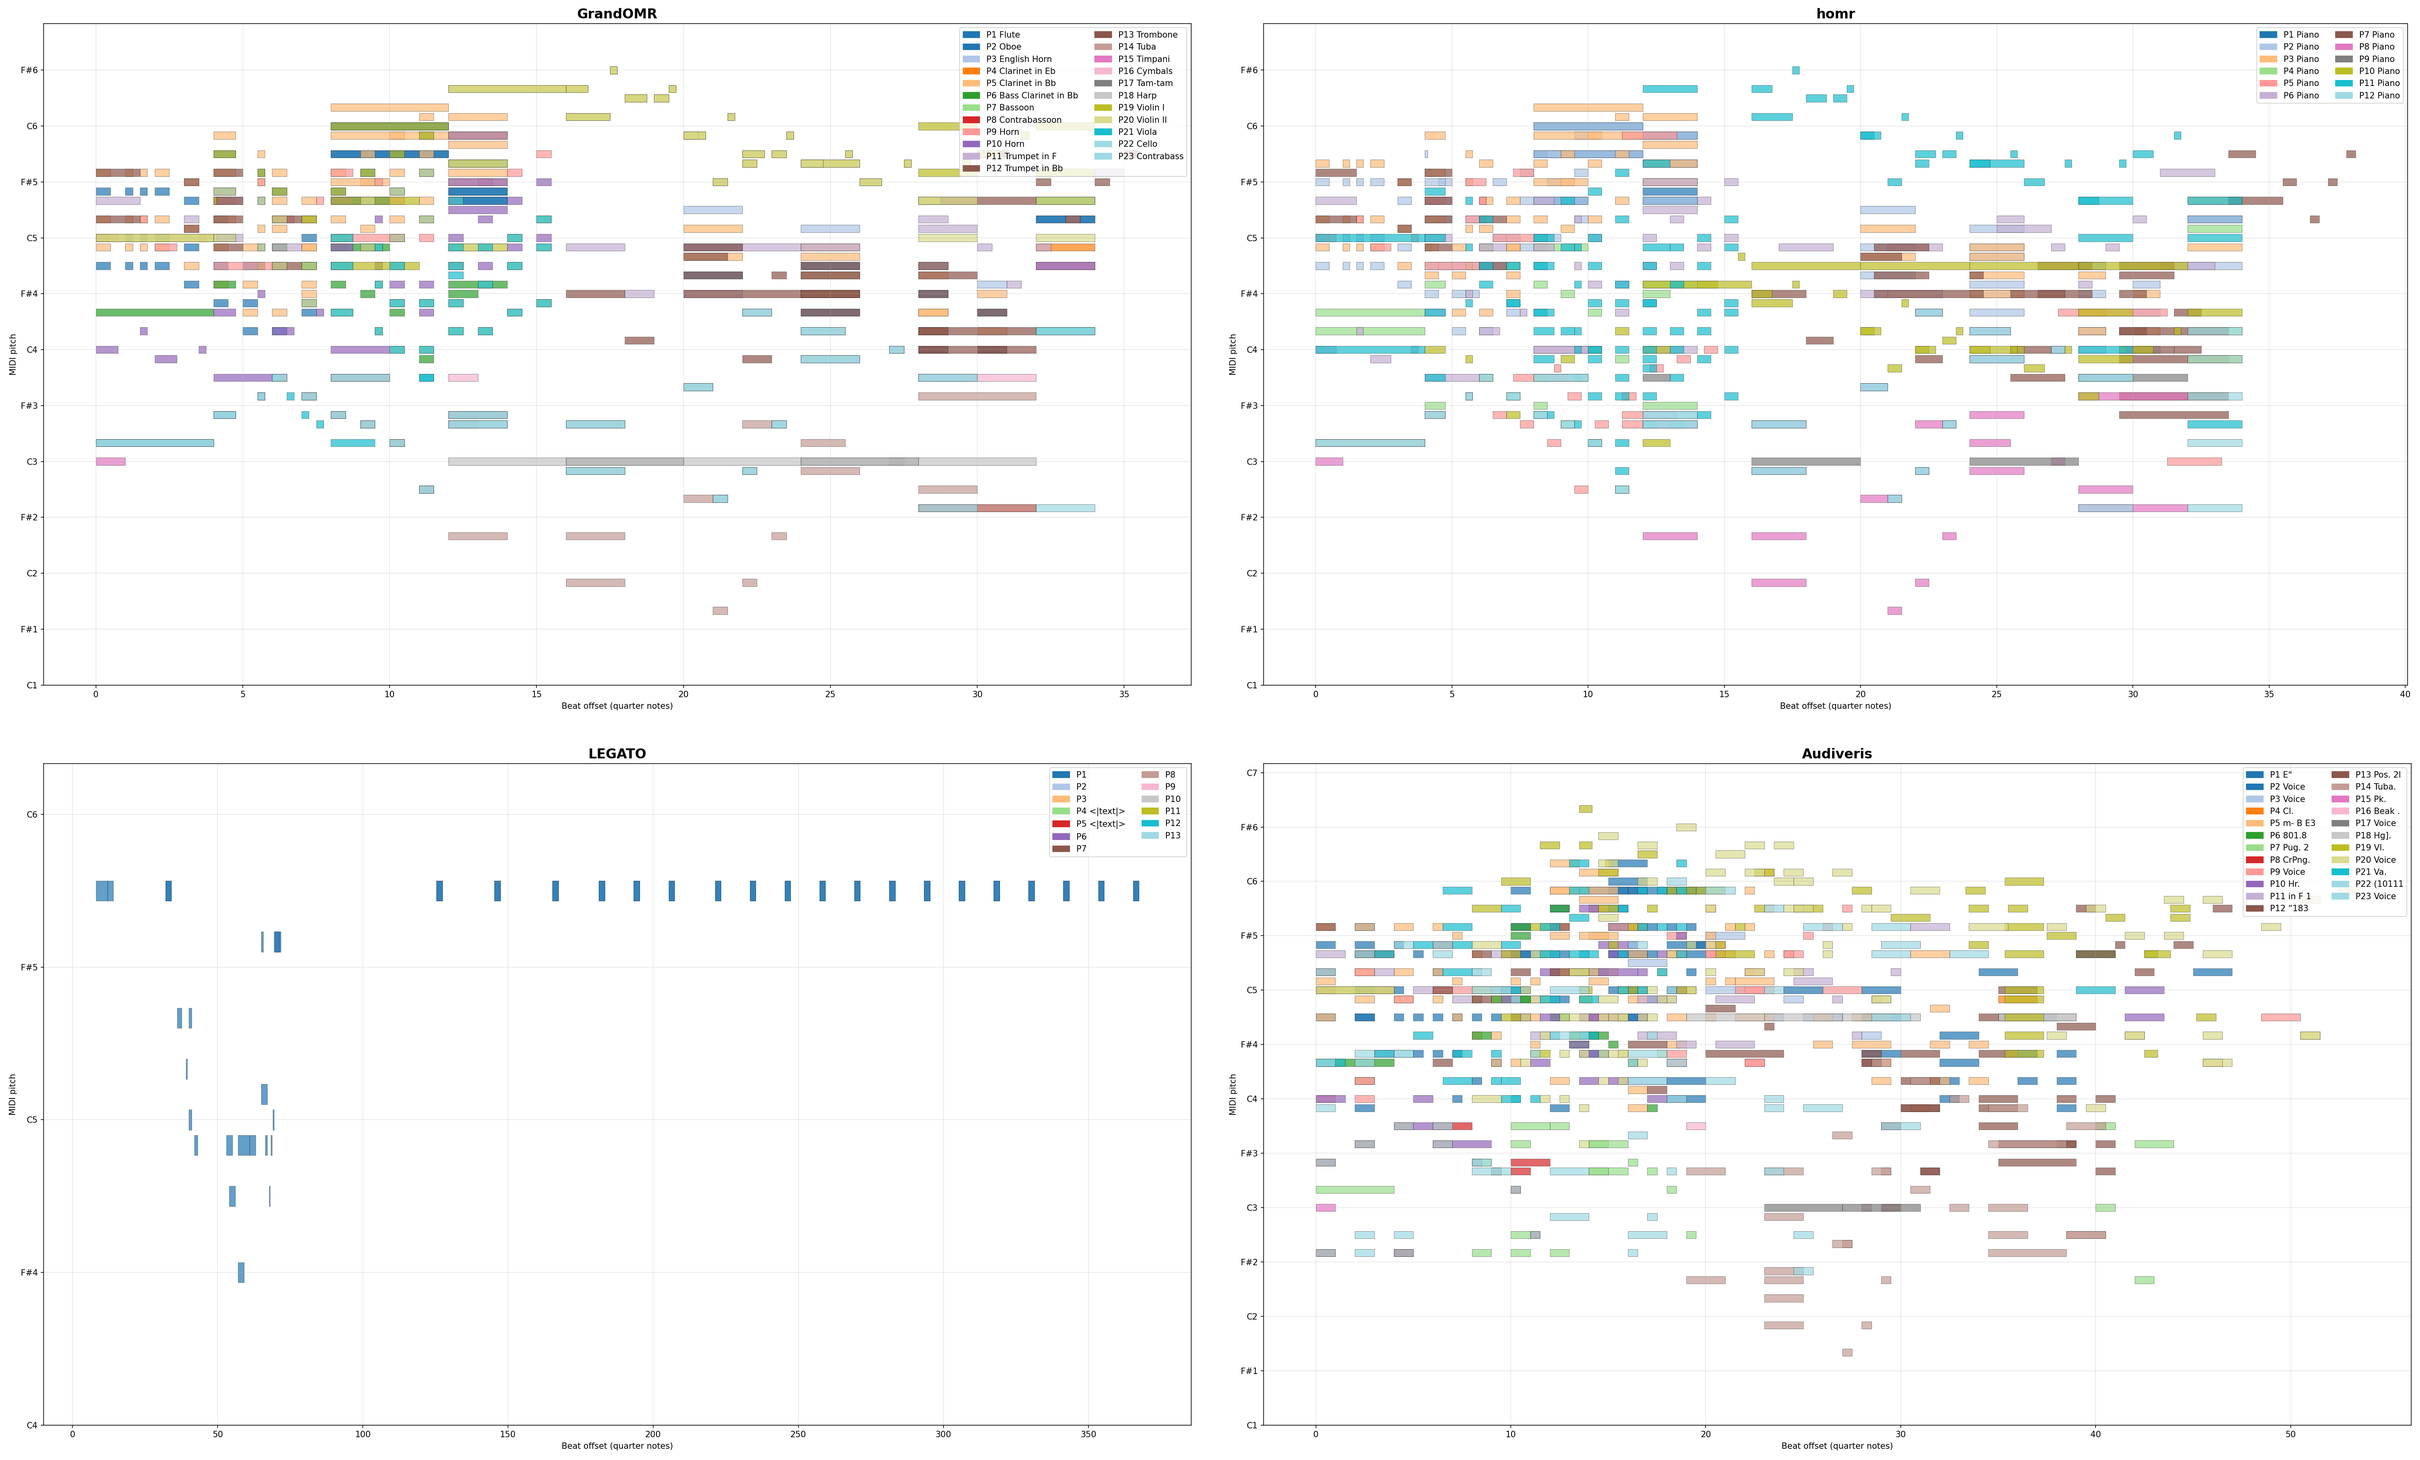
\includegraphics[width=\linewidth]{../outputs/Mahler7/page-255_comparison_2x2.png}
  \caption{Piano rolls for Mahler No.\,7, page~255 (2$\times$2 grid).
  \emph{Top-left:} GrandOMR (23 named parts, 366 notes).
  \emph{Top-right:} homr (12 unnamed Piano parts, 357 notes).
  \emph{Bottom-left:} LEGATO (13 parts, 60 notes — only first voice non-empty).
  \emph{Bottom-right:} Audiveris (23 parts, 318 notes, names garbled by OCR).}
  \label{fig:pr_compare}
\end{figure}

\subsection{Dynamics Detection}

\begin{table}[h]
\centering
\begin{tabular}{@{}lcccc@{}}
\toprule
 & No fine-tune & Fine-tune 30ep & Fine-tune 15ep \\
\midrule
mAP50 (all)          & 0.812 & 0.809 & \textbf{0.894} \\
mAP50 (dynamicF)     & 0.943 & 0.888 & \textbf{0.956} \\
mAP50 (dynamicP)     & 0.898 & 0.972 & \textbf{0.980} \\
mAP50 (dynamicS)     & 0.595 & 0.566 & \textbf{0.745} \\
\bottomrule
\end{tabular}
\caption{Dynamics detection mAP50. Fine-tuning 15 epochs outperforms 30 epochs
due to distribution shift when mosaic augmentation is disabled at epoch~21.}
\end{table}

The per-class confidence thresholds were chosen by inspecting the precision--recall curve of the 15-epoch model on the DeepScoresV2 dense test set.
Table~\ref{tab:dyn_thresh} summarises the precision and recall achieved at the selected operating point for the three classes with per-class thresholds.

\begin{table}[h]
\centering
\begin{tabular}{@{}lcccc@{}}
\toprule
Class & Threshold & Strategy & Precision & Recall \\
\midrule
dynamicF & 0.65 & Precision-first ($P \approx 0.95$) & $\approx 0.952$ & $\approx 0.875$ \\
dynamicP & 0.65 & Precision-first ($P \approx 0.95$) & $\approx 0.952$ & $\approx 0.875$ \\
dynamicS & 0.31 & Recall-first (F1-optimal) & 0.877 & 0.906 \\
\bottomrule
\end{tabular}
\caption{Confidence threshold selection for the three per-class dynamics classes.
\texttt{dynamicF} and \texttt{dynamicP} use precision-first thresholds to avoid spurious dynamics in playback.
\texttt{dynamicS} uses the F1-optimal threshold because sforzando markings only occur alongside $f$ or $p$, so slightly lower precision is acceptable.}
\label{tab:dyn_thresh}
\end{table}

\subsection{Qualitative Results}
% Piano roll visualizations: single page (Mahler 7 p.5, 17 parts, 5 measures)
%                            multi-page merge (pp.5-7, 23 parts, ~15 measures)

Figure~\ref{fig:pr_single} shows the piano roll for a single page of Mahler Symphony No.\,7
(page~5, 4/4, five measures).
GrandOMR correctly identifies all 17 instruments — including transposing instruments
(Clarinet in~A, Bass Clarinet in~A, Horn in~F) — and places notes within their expected
MIDI pitch ranges.
The quality checker reports one residual duration error in Violin~II, measure~4
(duration 5.0 instead of 4.0), illustrating the kind of minor inaccuracy that remains
after Layer~3 repair.

\begin{figure}[htbp]
  \centering
  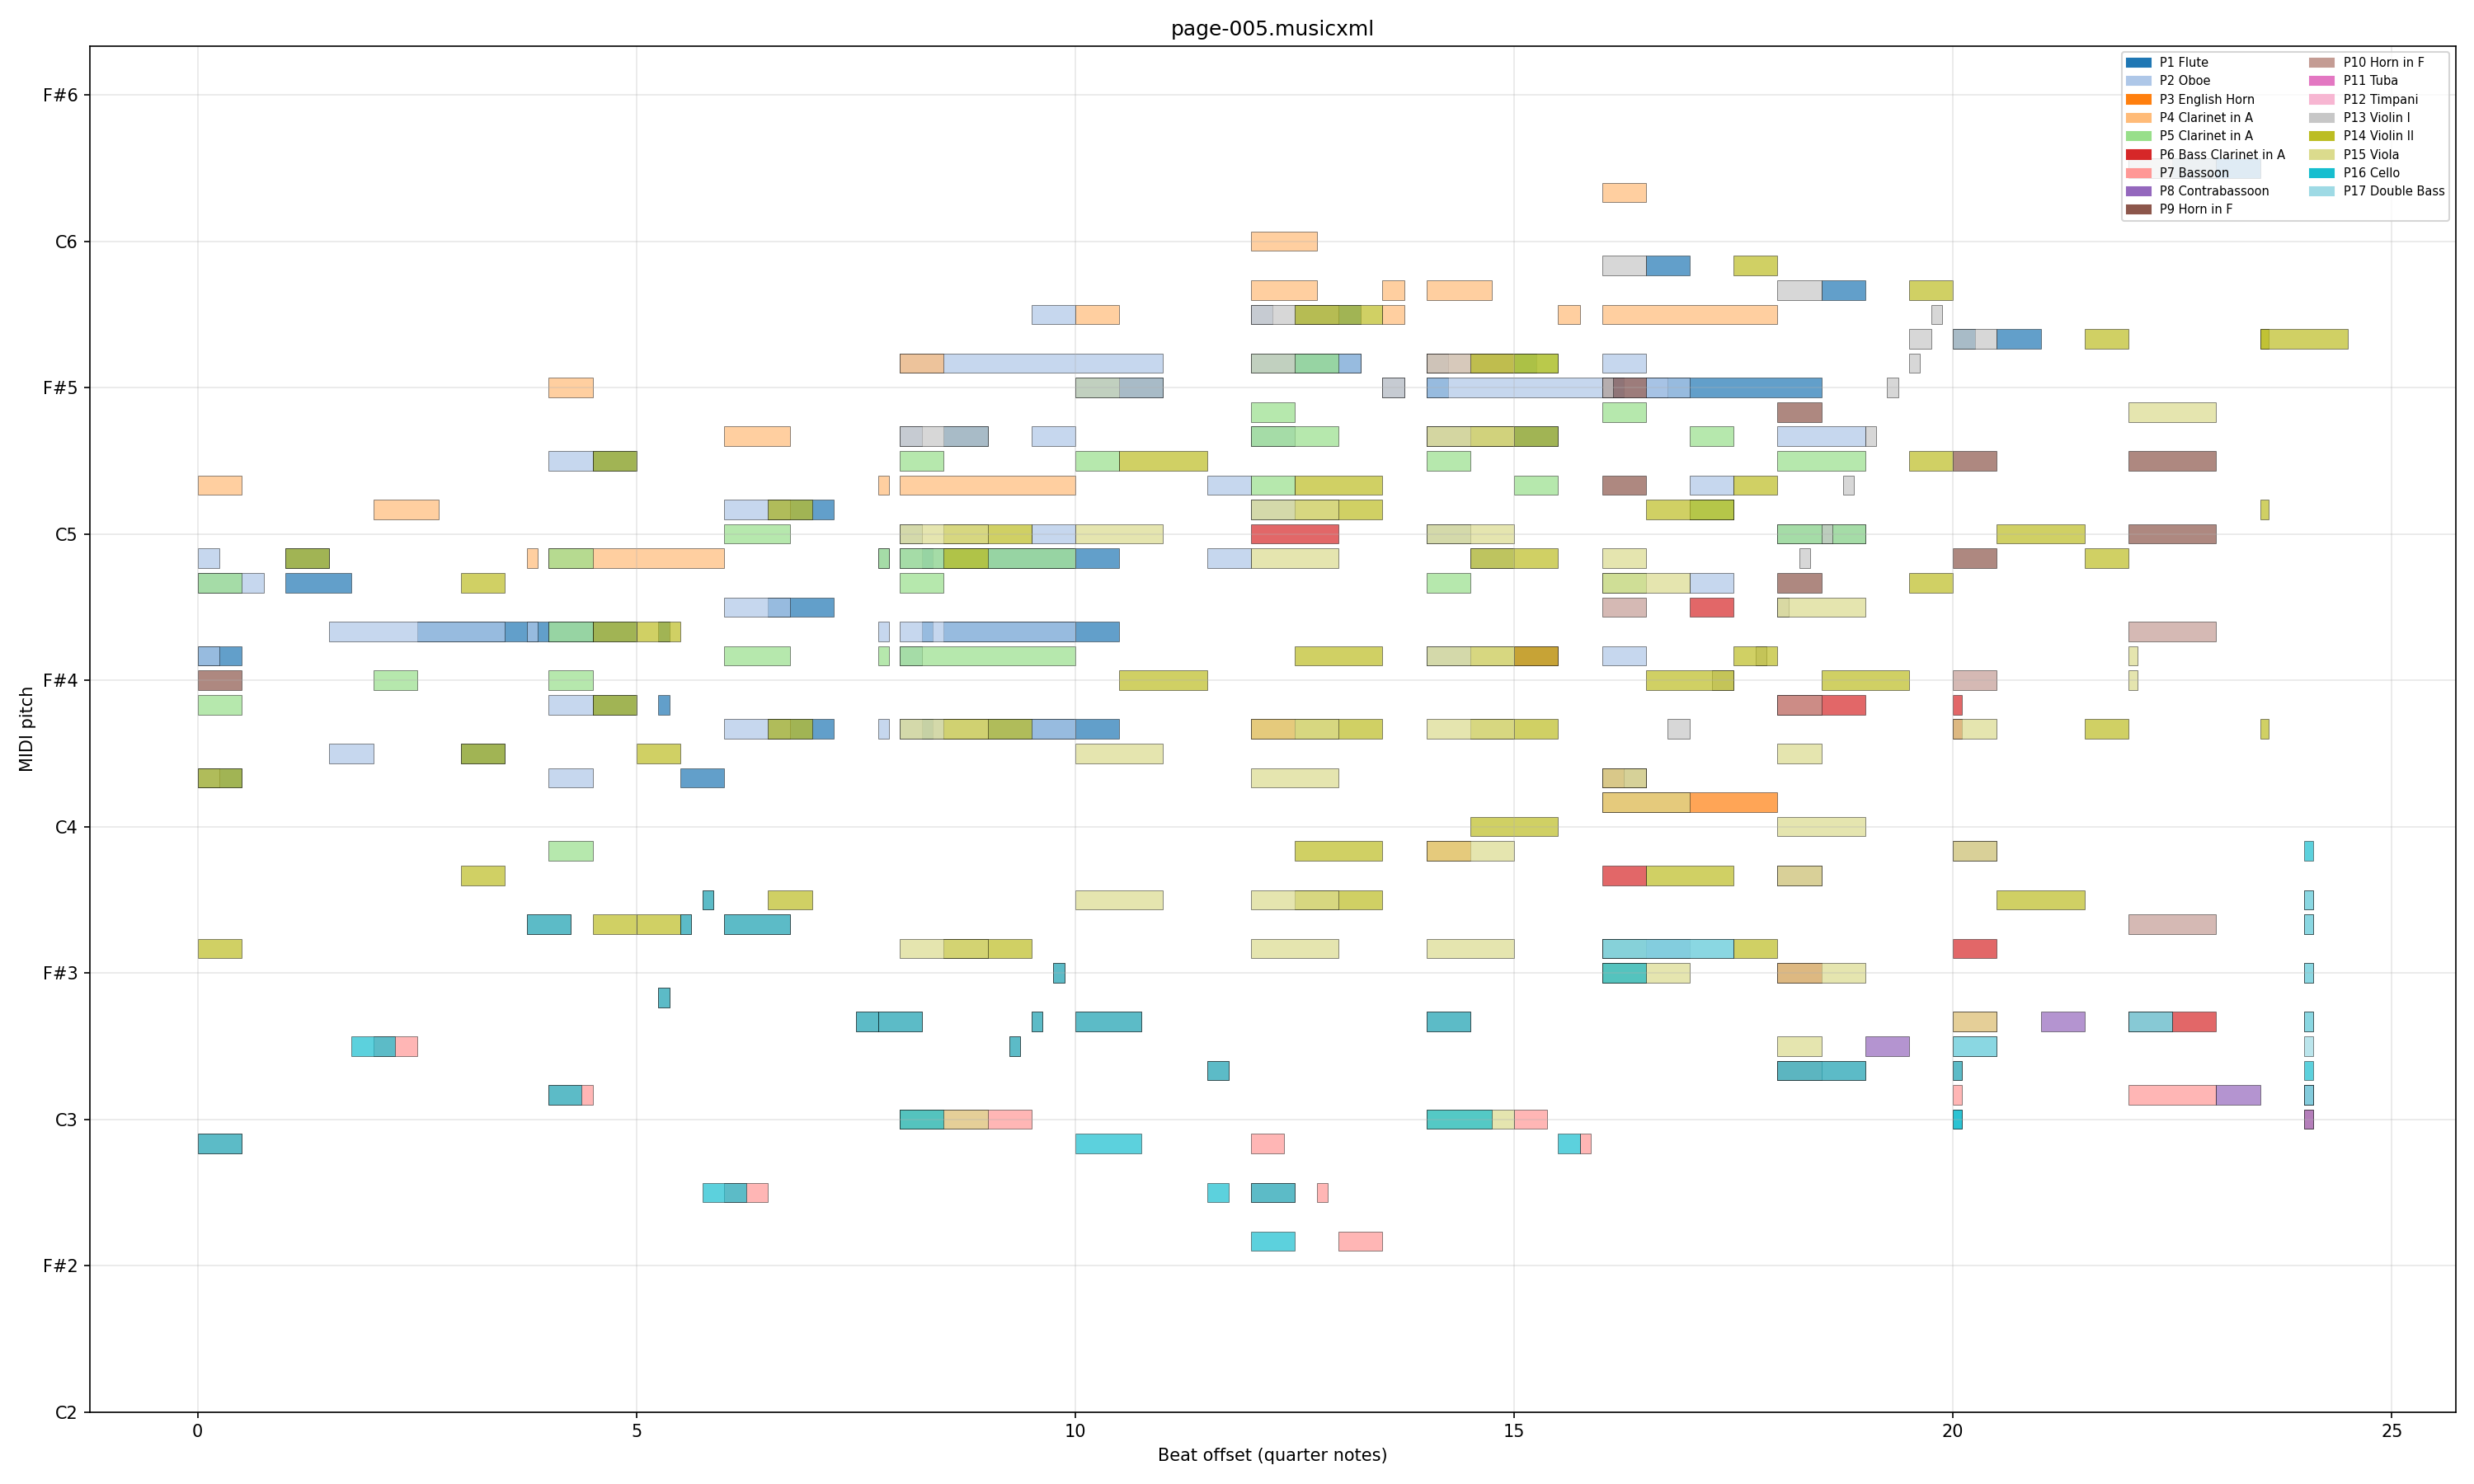
\includegraphics[width=\linewidth]{../examples/page-005_pianoroll.png}
  \caption{Piano roll for Mahler No.\,7, page~5 (single page, 17 parts, 5 measures).
  Each colour represents one instrument part; block width encodes note duration.}
  \label{fig:pr_single}
\end{figure}

Figure~\ref{fig:pr_merged} shows the result after merging pages~5–7.
The three-page output contains 23 parts, reflecting additional brass instruments
(Trombones, Tuba, Trumpet) that enter on page~6.
Cross-page name propagation correctly unifies the part list, and \texttt{ts\_context}
keeps time and key signatures consistent at page boundaries.
Minor issues include one Tuba note slightly above its standard range and two
additional duration errors in the string section, consistent with TrOMR's
known difficulty on fast passage-work.

\begin{figure}[htbp]
  \centering
  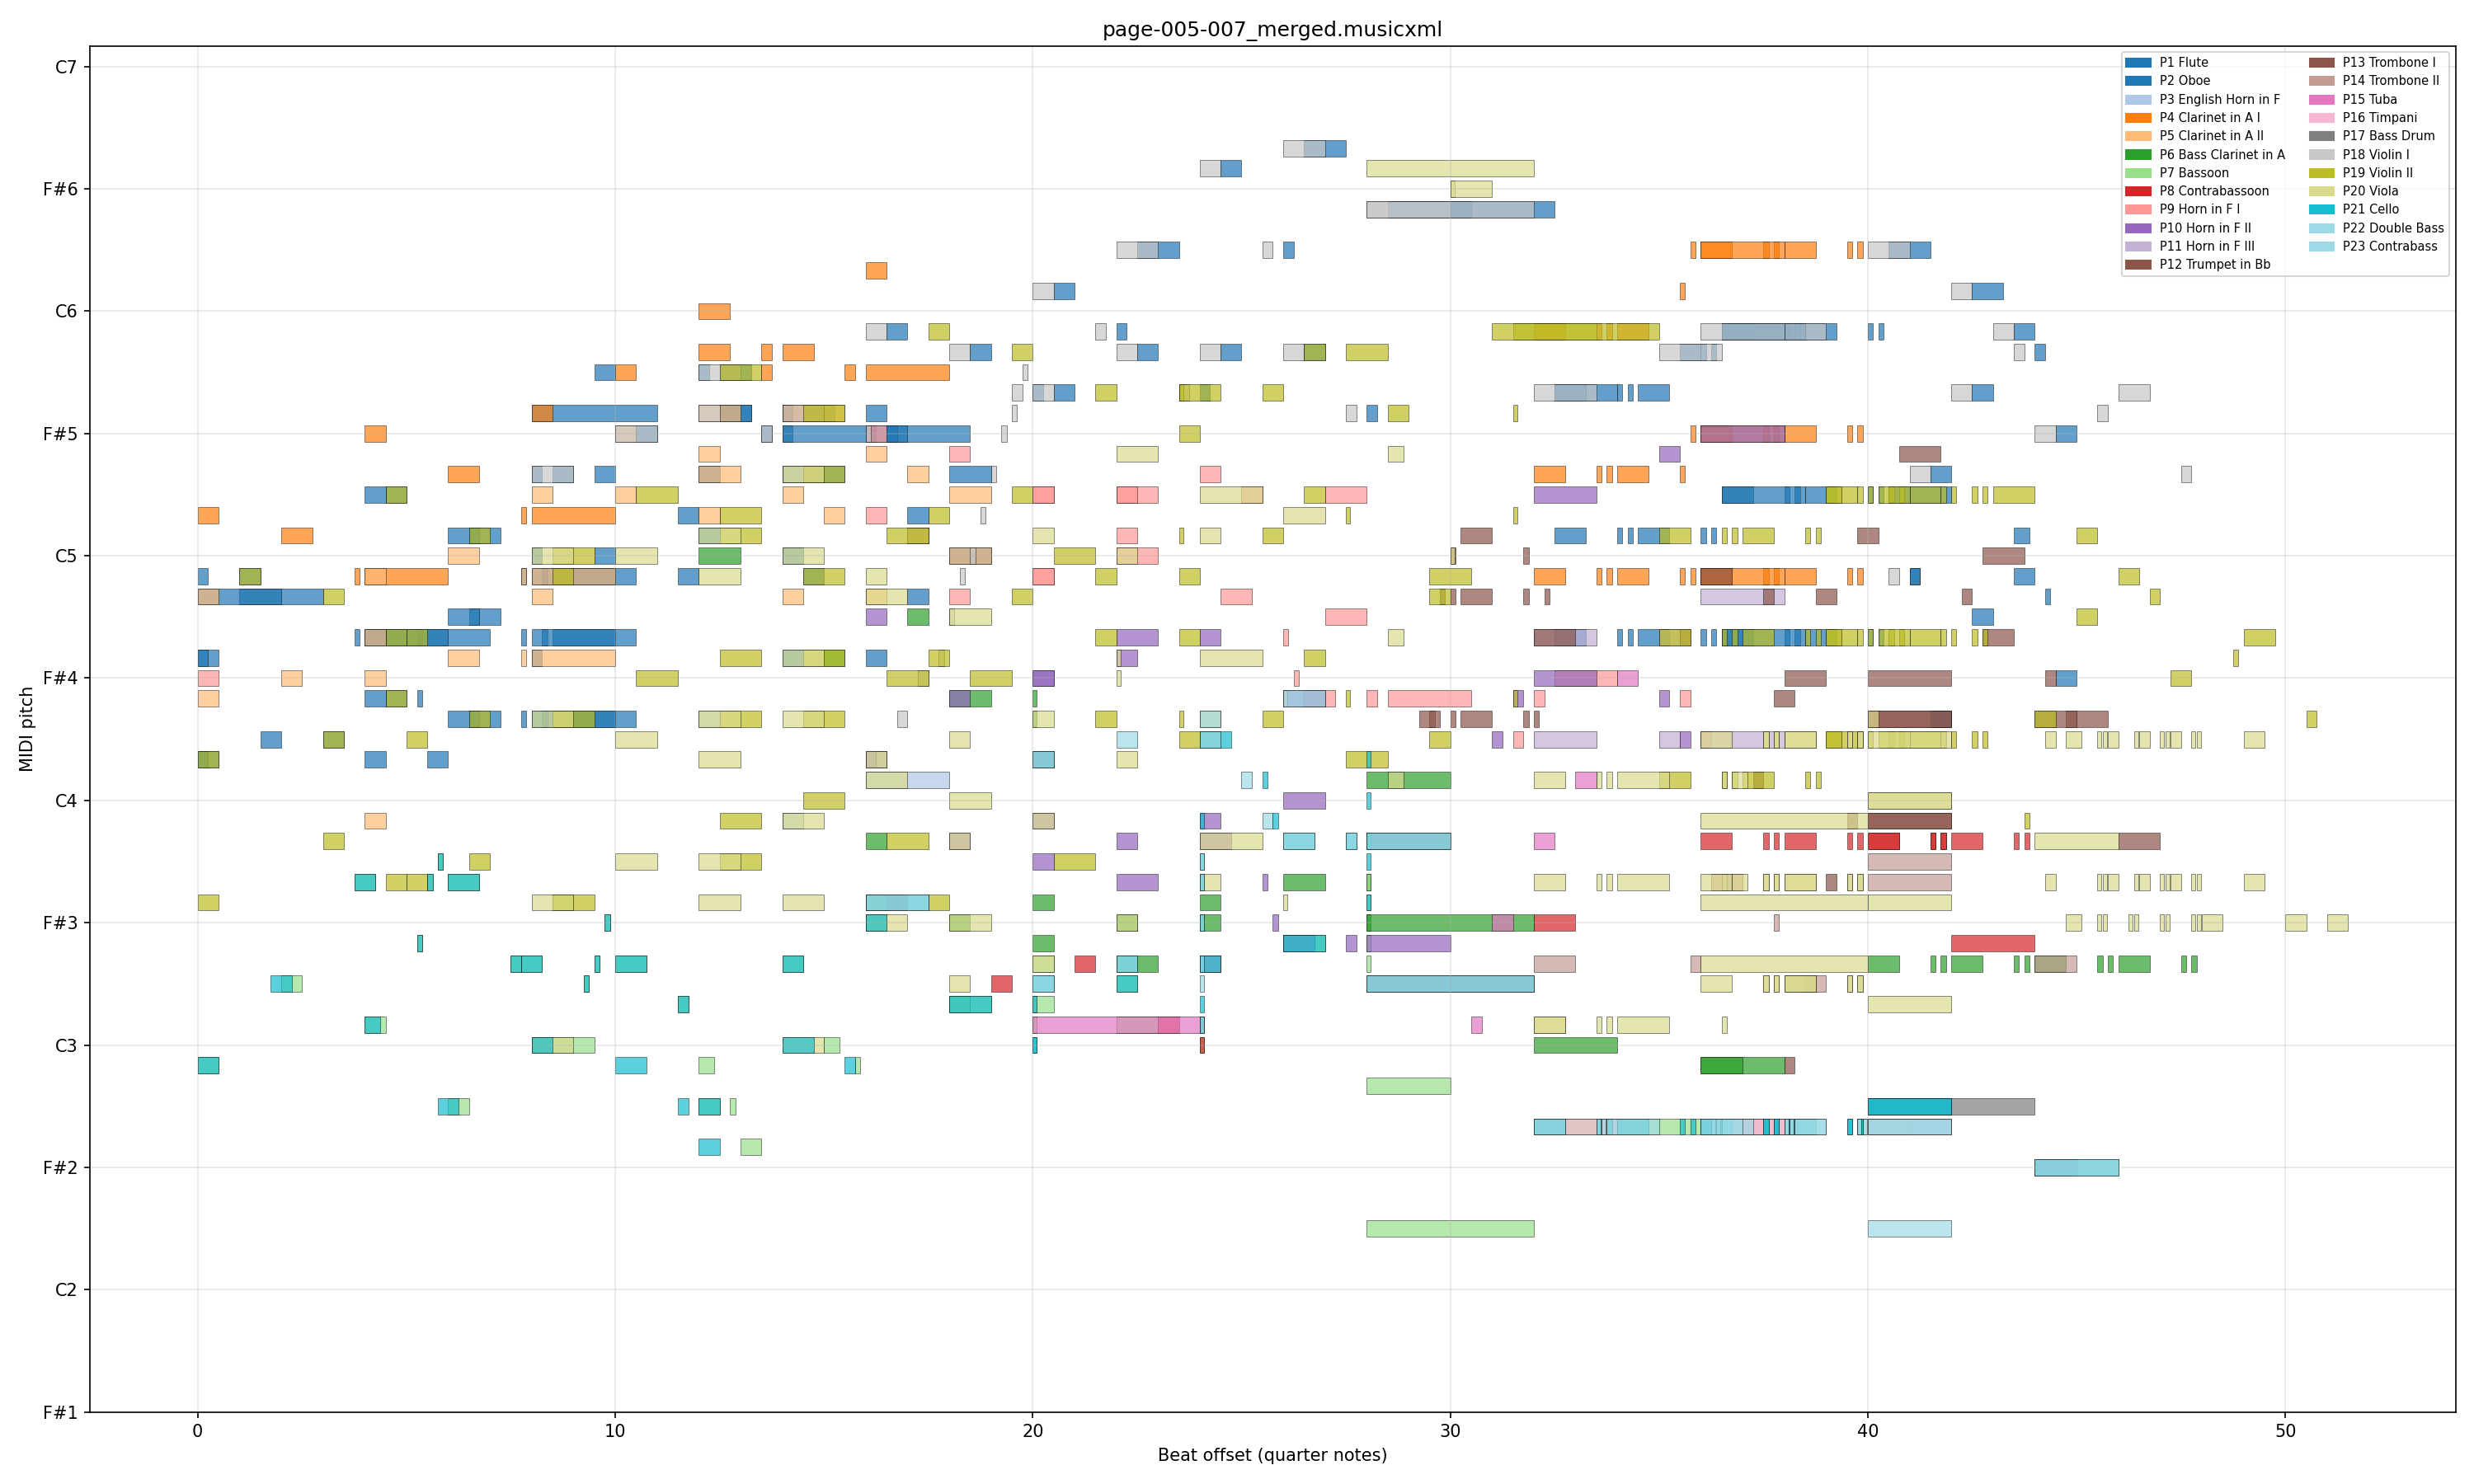
\includegraphics[width=\linewidth]{../examples/page-005-007_merged_pianoroll.png}
  \caption{Piano roll for Mahler No.\,7, pages~5–7 (multi-page merge, 23 parts, $\approx$15 measures).
  New instruments entering on page~6 are correctly appended to the unified part list.}
  \label{fig:pr_merged}
\end{figure}


% ─────────────────────────────────────────────────────────────────────────────
\section{Limitations and Future Work}
% ─────────────────────────────────────────────────────────────────────────────

% Main bottleneck: TrOMR per-staff recognition accuracy is limited,
%   requiring heavy rule-based post-processing that may introduce new errors
%   and increases processing time.
% Future: higher-accuracy single-staff model, or end-to-end multi-staff model
%   trained on manually corrected data.

The primary limitation of GrandOMR is the recognition accuracy of TrOMR, the per-staff sequence model at the core of Stage~2.
TrOMR operates independently on each staff, so errors in pitch, duration, or barline placement are common, particularly on complex rhythmic figures, beamed groups, and low-resolution scans.
These errors propagate downstream and necessitate the multi-layer rule-based post-processing described in Stage~3 — a substantial engineering effort whose repair heuristics may themselves introduce secondary errors or overcorrect in edge cases.
The overall effect is that the accuracy ceiling of the pipeline is set by TrOMR, and the complexity of Stage~3 is a direct consequence of that ceiling.

The most impactful direction for future work is therefore to raise per-staff recognition accuracy.
Two complementary approaches are promising.
First, a higher-accuracy single-staff model — whether through fine-tuning TrOMR on a larger or more diverse dataset, or adopting a more capable architecture — would reduce the burden on post-processing and improve output quality directly.
Second, an end-to-end multi-staff model trained on manually corrected full-system transcriptions could bypass the per-staff decomposition entirely, allowing the model to exploit cross-staff harmonic and rhythmic context that is invisible to a per-staff approach.


% ─────────────────────────────────────────────────────────────────────────────
\section{Conclusion}
% ─────────────────────────────────────────────────────────────────────────────

% Restate core design principle: matching each subproblem to the most suitable
% CV method (semantic segmentation / VLM / Transformer / object detection /
% domain rules) yields a pipeline that is more interpretable and controllable
% than a monolithic end-to-end approach, and achieves competitive results on
% full orchestral scores.

We have presented GrandOMR, a hybrid OMR pipeline for full orchestral scores built around a single design principle: decompose the recognition task into its constituent subproblems and match each to the most appropriate computer vision method.
Pixel-level semantic segmentation handles the regular geometric structure of stave detection; a two-pass vision-language model handles the open-vocabulary, multilingual challenge of instrument name reading; a Transformer encoder-decoder handles the sequence transduction nature of per-staff note recognition; rule-based post-processing exploits the well-defined consistency constraints shared by all parts of an orchestral score; and a fine-tuned object detector handles the fixed-vocabulary local-pattern nature of dynamics detection.
This decomposition yields a pipeline that is more interpretable and controllable than a monolithic end-to-end approach: each component can be inspected, replaced, or improved independently, and domain knowledge can be incorporated directly as rules without retraining.
Experiments on IMSLP orchestral scans demonstrate that GrandOMR achieves competitive results on full scores that current end-to-end systems cannot handle, while preserving instrument identity, transposition, dynamics, and cross-page structural context that are essential for interactive playback.


\begin{thebibliography}{9}
\bibitem{imslp} International Music Score Library Project (IMSLP). \url{https://imslp.org}.
\bibitem{audiveris} Audiveris OMR Engine. \url{https://github.com/Audiveris/audiveris}.
\bibitem{tromr} Z.~Li et al., ``TrOMR: Transformer-based Polyphonic Optical Music Recognition,'' \textit{ICASSP}, 2023.
\bibitem{oemer} Yoyo et al., ``BreezeWhite/oemer: v0.1.7,'' Zenodo, 2023. \textit{homr}: \url{https://github.com/liebharc/homr}.
\bibitem{legato} G.~Yang et al., ``LEGATO: Large-scale End-to-end Generalizable Approach to Typeset OMR,'' \textit{arXiv:2506.19065}, 2025.
\bibitem{qwen3vl} Qwen Team, ``Qwen3 Technical Report,'' Alibaba Cloud, \textit{arXiv:2505.09388}, 2025.
\bibitem{rapidocr} RapidAI, ``RapidOCR: A Lightweight, Fast and Accurate OCR Engine,'' 2022. \url{https://github.com/RapidAI/RapidOCR}.
\end{thebibliography}

\end{document}
